\documentclass[aspectratio=169, 11pt]{beamer}

% Tema minimalista moderno
\usetheme{default}
\useinnertheme{rectangles}

% Remover barras de navegação superior e símbolos
\setbeamertemplate{navigation symbols}{}
\setbeamertemplate{headline}{}

% Cores modernas de alto contraste
\definecolor{primary}{HTML}{14213D}      % Azul Escuro
\definecolor{secondary}{HTML}{FCA311}    % Ouro/Amarelo Moderno
\definecolor{accent}{HTML}{E76F51}       % Laranja/Terracota
\definecolor{bglight}{HTML}{F8F9FA}      % Fundo Off-White
\definecolor{textdark}{HTML}{212529}     % Texto Escuro

\setbeamercolor{background canvas}{bg=bglight}
\setbeamercolor{normal text}{fg=textdark}
\setbeamercolor{structure}{fg=primary}
\setbeamercolor{item}{fg=secondary}

% Título de Frame limpo e elegante
\setbeamercolor{frametitle}{bg=bglight, fg=primary}
\setbeamerfont{frametitle}{size=\Large, series=\bfseries}
\setbeamertemplate{frametitle}{
  \vspace{0.6cm}
  \insertframetitle
  \par\vskip-6pt
}

% Blocos planos
\setbeamertemplate{blocks}[rounded][shadow=false]
\setbeamercolor{block title}{bg=primary, fg=white}
\setbeamercolor{block body}{bg=white, fg=textdark}

% Marcadores de listas
\setbeamertemplate{itemize item}{\color{accent}$\bullet$}
\setbeamertemplate{itemize subitem}{\color{primary}$\circ$}

% Rodapé contendo apenas número de slides
\setbeamertemplate{footline}{
  \hfill
  \begin{beamercolorbox}[wd=0.1\paperwidth,ht=2.25ex,dp=1ex,right,rightskip=3ex]{normal text}
    \usebeamerfont{date in head/foot}\color{primary!50}\insertframenumber{} / \inserttotalframenumber
  \end{beamercolorbox}
  \vspace{0.4cm}
}

\usepackage[utf8]{inputenc}
\usepackage[T1]{fontenc}
\usepackage[brazil]{babel}
\usepackage{graphicx}
\graphicspath{{../}}
\usepackage{booktabs}
\usepackage{amsmath}
\usepackage{amsfonts}

\title[Validação de Trabalhos Futuros]{Implementação e Validação de Trabalhos Futuros no ClonalG}
\subtitle{Decaimento Dinâmico de Mutação e Métrica Davies-Bouldin}
\author[Marcos e Vinicius]{Marcos Daniel e Vinicius Macedo}
\institute[IFNMG]{Instituto Federal do Norte de Minas Gerais}
\date{Julho de 2026}

\begin{document}

\begin{frame}
  \titlepage
\end{frame}

\begin{frame}{Introdução}
  \begin{itemize}
    \item \textbf{Contexto:} As melhorias do Lab 4 trouxeram busca espacial contínua e diversidade, mas identificou-se espaço para otimização em dois eixos (Trabalhos Futuros):
      \begin{itemize}
        \item \textbf{Ajuste Fino de Convergência:} Parâmetros fixos de mutação causam oscilação em torno do ótimo final (falta de decaimento).
        \item \textbf{Métricas Alternativas de Afinidade:} O Índice Silhouette é computacionalmente proibitivo para grandes datasets e sensível a ruídos geométricos.
      \end{itemize}
    \item \textbf{Objetivo do Trabalho:} Implementar decaimento dinâmico de hipermutação e a métrica Davies-Bouldin como afinidade, comparando com as versões anteriores.
  \end{itemize}
\end{frame}

\begin{frame}{O Algoritmo ClonalG (Breve Recomposição)}
  \begin{itemize}
    \item \textbf{Sistema Imunológico Artificial (SIA):}
      \begin{itemize}
        \item \textbf{Reconhecimento:} Anticorpos representam conjuntos de centroides avaliados por afinidade.
        \item \textbf{Proliferação:} Clones são gerados proporcionalmente à sua afinidade de clustering.
        \item \textbf{Hipermutação Somática:} Mutações inversamente proporcionais à afinidade.
        \item \textbf{Seleção de Memória:} Melhores soluções são salvas; piores são substituídas por novos anticorpos aleatórios.
      \end{itemize}
  \end{itemize}
\end{frame}

\begin{frame}{Proposta de Melhoria 1: Decaimento Dinâmico de Mutação}
  \begin{itemize}
    \item \textbf{Problema Anterior:} O tamanho da mutação paramétrica $\sigma$ e a probabilidade de mutação estrutural $\alpha$ mantinham-se constantes. Isso gerava instabilidade no final da busca (convergência oscilatória).
    \item \textbf{Mecanismo Adotado:} Fator de decaimento linear da geração atual $it$ sobre $n\_iterations$:
      \[ \text{decay} = \max\left(0.05, 1.0 - \frac{it}{n\_iterations}\right) \]
    \item \textbf{Aplicações do Decaimento:}
      \begin{itemize}
        \item \textbf{Estrutural:} $\alpha_{\text{novo}} = \alpha \times \text{decay}$ (foca em manter $k$ estável nas últimas gerações).
        \item \textbf{Espacial:} $\sigma_{\text{novo}} = \sigma \times \text{decay}$ (refina a posição exata dos centroides).
      \end{itemize}
  \end{itemize}
\end{frame}

\begin{frame}{Proposta de Melhoria 2: Afinidade via Davies-Bouldin}
  \begin{itemize}
    \item \textbf{Davies-Bouldin (DB) como Afinidade:}
      \begin{itemize}
        \item Avalia a similaridade entre clusters com base na dispersão interna ($S_i$) e na separabilidade entre eles ($d(c_i, c_j)$).
        \item Como DB é um índice a ser minimizado, definimos a afinidade como o seu oposto:
          \[ A = - DB = - \frac{1}{k} \sum_{i=1}^{k} \max_{j \neq i} \left( \frac{S_i + S_j}{d(c_i, c_j)} \right) \]
      \end{itemize}
    \item \textbf{Vantagem Computacional:} Davies-Bouldin exige apenas a distância dos pontos aos centroides do seu próprio grupo e as distâncias mútuas entre os centroides. A complexidade é linear em relação ao número de pontos ($O(N)$), enquanto o Silhouette é quadrático ($O(N^2)$).
  \end{itemize}
\end{frame}

\begin{frame}{Comparação de Resultados: Silhouette Médio}
  \begin{table}
    \centering
    \footnotesize
    \begin{tabular}{lccccc}
      \toprule
      Variante / Algoritmo & DS1 & DS2 & DS3 & DS4 & DS5 \\
      \midrule
      ClonalG Clássico (Lab 2) & 0.6480 & 0.6285 & 0.1979 & 0.5875 & 0.6644 \\
      ClonalG Otimizado (Lab 4) & 0.6480 & 0.6158 & \textbf{0.2032} & \textbf{0.5902} & 0.6644 \\
      \textbf{ClonalG com Decaimento (Sil)} & 0.6480 & \textbf{0.6539} & 0.1972 & \textbf{0.5902} & 0.6644 \\
      ClonalG com Decaimento (DB) & 0.6480 & 0.6253 & 0.1650 & 0.5790 & 0.6644 \\
      \bottomrule
    \end{tabular}
    \caption{Silhouette médio comparativo (maior é melhor) em 3 runs.}
  \end{table}
  \begin{itemize}
    \item \textbf{Destaque no DS2:} A introdução do decaimento dinâmico de mutação elevou a média de Silhouette para \textbf{0.6539}, o melhor resultado entre todas as versões.
  \end{itemize}
\end{frame}

\begin{frame}{Comparação de Resultados: Davies-Bouldin Médio}
  \begin{table}
    \centering
    \footnotesize
    \begin{tabular}{lccccc}
      \toprule
      Variante / Algoritmo & DS1 & DS2 & DS3 & DS4 & DS5 \\
      \midrule
      ClonalG Clássico (Lab 2) & 0.4837 & 0.4949 & 1.5833 & 0.5397 & 0.5046 \\
      ClonalG Otimizado (Lab 4) & 0.4837 & 0.5454 & 1.3903 & 0.5323 & 0.5046 \\
      ClonalG com Decaimento (Sil) & 0.4837 & \textbf{0.3939} & 1.4307 & 0.5347 & 0.5046 \\
      \textbf{ClonalG com Decaimento (DB)} & 0.4837 & 0.5161 & \textbf{1.3039} & \textbf{0.5312} & 0.5046 \\
      \bottomrule
    \end{tabular}
    \caption{Davies-Bouldin médio comparativo (menor é melhor) em 3 runs.}
  \end{table}
  \begin{itemize}
    \item \textbf{Destaque nos DS3 e DS4:} A otimização direta pelo índice Davies-Bouldin resultou nos menores índices de espalhamento obtidos (\textbf{1.3039} e \textbf{0.5312}, respectivamente).
  \end{itemize}
\end{frame}

\begin{frame}{Comportamento de Convergência da Afinidade}
  \begin{columns}
    \begin{column}{0.6\textwidth}
      \begin{center}
        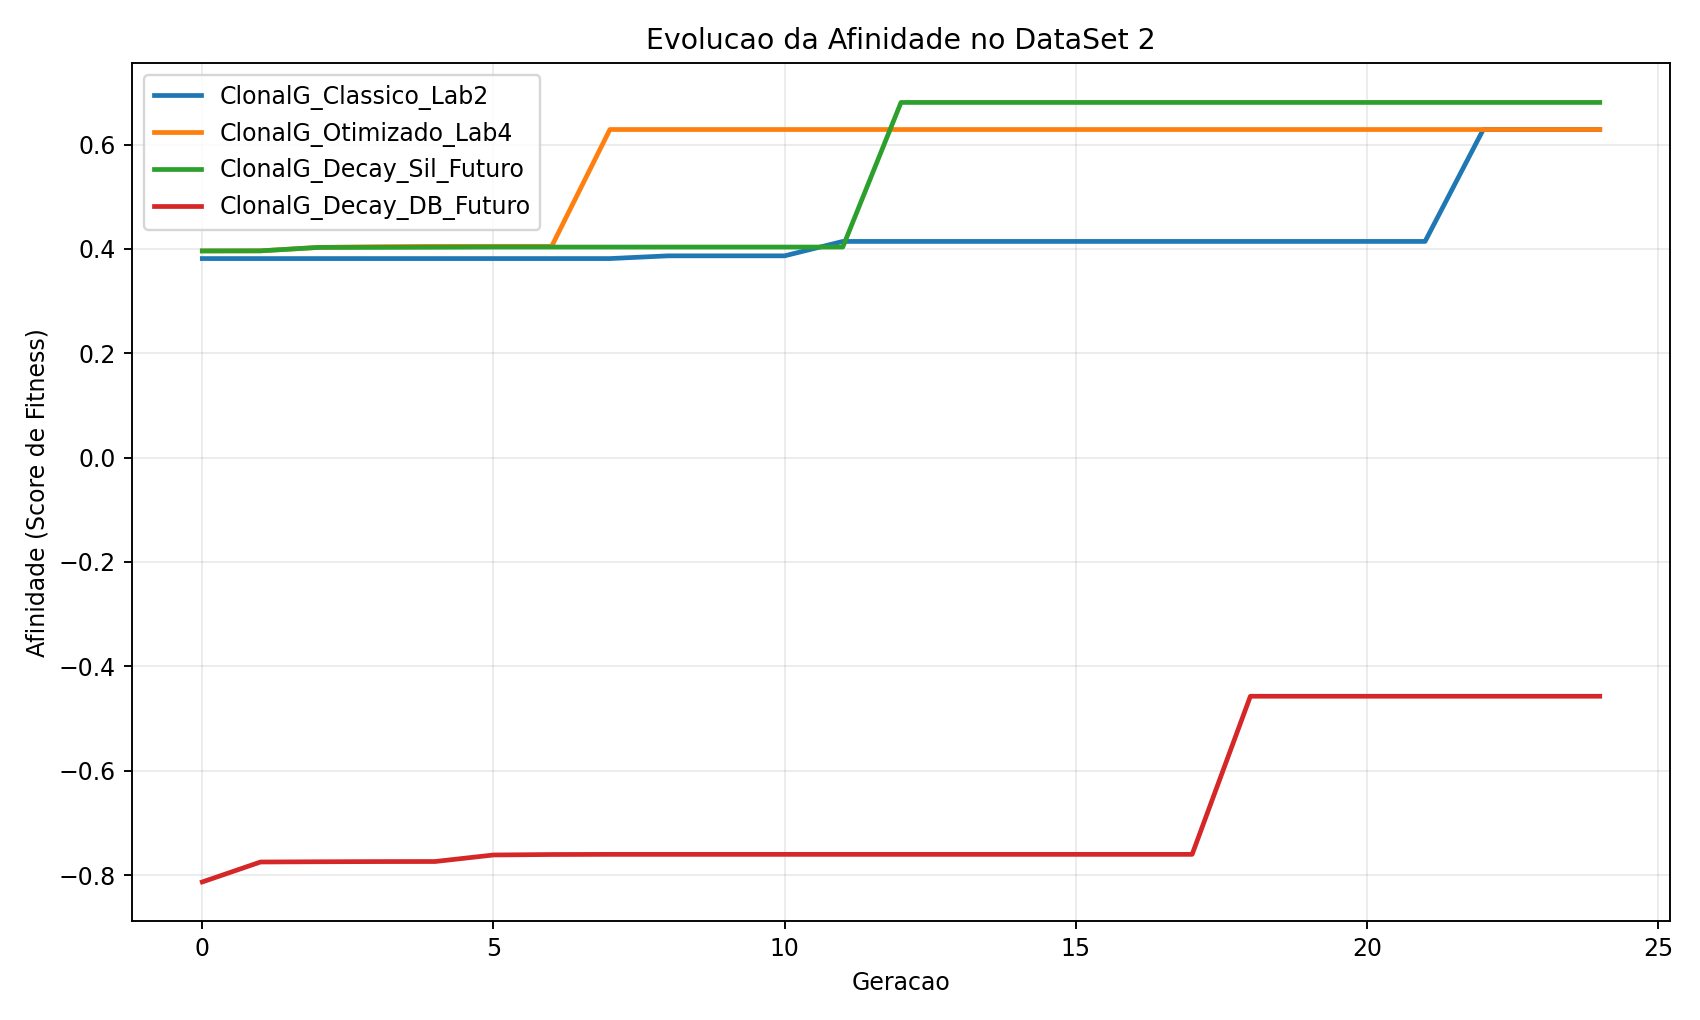
\includegraphics[width=0.9\textwidth]{resultados/comparativo_trabalhos_futuros/evolucao_ds2.png}
      \end{center}
    \end{column}
    \begin{column}{0.4\textwidth}
      \textbf{Análise das Curvas no DS2:}
      \begin{itemize}
        \item O \textbf{ClonalG com Decaimento (Sil)} atinge a convergência de maneira mais rápida e estável.
        \item O \textbf{ClonalG Otimizado (Lab 4)} oscila por falta de resfriamento de mutação.
        \item O \textbf{ClonalG com Decaimento (DB)} maximiza a afinidade rapidamente mas sob uma métrica distinta (o que desloca a curva de Silhouette).
      \end{itemize}
    \end{column}
  \end{columns}
\end{frame}

\begin{frame}{Conclusões}
  \begin{itemize}
    \item \textbf{Eficácia do Decaimento Dinâmico:}
      \begin{itemize}
        \item Reduzir a taxa de mutação com o tempo evitou dispersão nas gerações finais, permitindo que a busca local estabilizasse os centroides no pico ótimo do Silhouette.
      \end{itemize}
    \item \textbf{Viabilidade do Davies-Bouldin:}
      \begin{itemize}
        \item A otimização pelo índice DB resultou em agrupamentos compactos e robustos (comprovado pelos ótimos índices DB alcançados), com a grande vantagem de requerer apenas uma fração do tempo de cálculo computacional do Silhouette.
      \end{itemize}
    \item \textbf{Resumo:} As propostas de trabalhos futuros implementadas tornaram o ClonalG mais estável, mais rápido e teoricamente apto a lidar com datasets ainda maiores.
  \end{itemize}
\end{frame}

\end{document}
